\documentclass[accentcolor=tud0b,12pt,paper=a4]{tudreport}

\usepackage[utf8]{inputenc}
\usepackage{ngerman}
\usepackage{parcolumns}
\usepackage{hyperref}
\usepackage{multicol}
\usepackage{pdfpages}


\setlength{\parindent}{0pt}
\setlength{\parskip}{1em}

\newcommand{\titlerow}[2]{
	\begin{parcolumns}[colwidths={1=.2\linewidth}]{2}
		\colchunk[1]{#1:}
		\colchunk[2]{#2}
	\end{parcolumns}
	\vspace{0.15cm}
}

\title{CloneCademy}
\subtitle{Qualitätssicherungsdokument}
\subsubtitle{%
	\titlerow{Gruppe 12}{%
		Ilhan Simsiki
		<\href{mailto:ilhan.simsiki@stud.tu-darmstadt.de}{ilhan.simsiki@stud.tu-darmstadt.de}>\\
		Leonhard Wiedmann
		<\href{mailto:leonhard.wiedmann@stud.tu-darmstadt.de}{leonhard.wiedmann@stud.tu-darmstadt.de}>\\
		Tobias Huber
		<\href{mailto:tobias.huber@stud.tu-darmstadt.de}{tobias.huber@stud.tu-darmstadt.de}>\\
		Claas Völcker
		<\href{mailto:c.voelcker@stud.tu-darmstadt.de}{c.voelcker@stud.tu-darmstadt.de}>}
	\titlerow{Teamleiter}{Alexander Nagl
		<\href{mailto:alexander.nagl@t-online.de}{alexander.nagl@t-online.de}>}
	\titlerow{Auftraggeber}{%
		iGEM-Team TU Darmstadt\\
		vertreten durch Thea Lotz <\href{mailto:lotz@bio.tu-darmstadt.de}{lotz@bio.tu-darmstadt.de}>\\
		Fachbereich Biologie}
	\titlerow{Abgabedatum}{14.07.2017}}
\institution{Bachelor-Praktikum SoSe 2017\\Fachbereich Informatik}

\begin{document}

\maketitle
\tableofcontents

\chapter*{Anmerkungen und Hinweise}
Die Verfasser dieses Dokumentes verwenden als Maßnahme für die Gleichstellung aller Personen die sogenannte "`gendergerechte Sprache"'. Als Zeichen der Inklusion aller Geschlechter wird der Stern (*) oder eine Verlaufsform (\emph{Nutzung} statt \emph{Nutzer}) verwendet. Von dieser Regelung wird nur abgewichen, wenn entweder alle Mitglieder einer Gruppe sich ein und demselben Geschlecht zugehörig fühlen (z.B. im Entwicklerteam) oder die Vorgaben der Veranstalter*innen keine Alternative zulassen (z.B. auf dem Deckblatt).

\chapter{Einleitung}

\emph{CloneCademy} ist ein Projekt für das iGEM-Team der TU Darmstadt. Die \emph{international Genetically Engineered Machine competition} (iGEM) ist ein internationaler Wettbewerb für Studierende auf dem Gebiet der synthetischen Biologie.
Dieser wird seit 2003 von der iGEM-Foundation veranstaltet.

Im Rahmen des Wettbewerbs wird eine Online-Lernplattform für das iGEM-Team der TU Darmstadt erstellt. Das Ziel dieser Plattform ist es, durch interaktive Unterrichtseinheiten Prinzipien der Molekularbiologie sowie der synthetischen Biologie zu erlernen und sowohl eigene Lernfortschritte, als auch die anderer Teams begutachten zu können. Darüber hinaus soll es auch anderen Interessierten (z.B. andere iGEM-Teams, Lehrende an Universitäten und Schulen, etc.) möglich sein, eigene Inhalte einzupflegen und zur Verfügung zu stellen.

Als Kernfunktionalität bietet die Plattform Nutzer*innen die Möglichkeit, sich zu registrieren und einen Account anzulegen. Registrierte Nutzer*innen können bereitgestellte Aufgaben bearbeiten und Feedback zu ihren Antworten erhalten. Zusätzlich können Nutzer*innen mit Moderationsrechten neue Aufgaben in das System einpflegen und bereits bestehende überarbeiten. Die bereitgestellten Aufgabentypen sind Multiple-Choice-, Drag-And-Drop- und Lückentextaufgaben. Außerdem wird im Rahmen des vereinbarten Ziels der \emph{Veränderbarkeit} die Möglichkeit geschaffen, nach Ende des Projektes auch noch weiter Aufgabentypen in die Plattform einzubauen.

Um einen Überblick über ihren bisherigen Lernerfolg zu bekommen, haben Nutzer*innen die Möglichkeit, Statistiken zu ihrer Nutzung der Plattform einzusehen. Den Auftraggeber*innen geben diese Statistiken auch Einblick in die Nutzung und die Qualität ihrer Inhalte, so dass diese weiter verbessert werden können.

Das Ziel des Projektes ist eine voll funktionsfähige Webanwendung für die aktuellen Versionen der Browser \emph{Firefox} und \emph{Chrome} auf Desktop- und Laptoprechner bereitzustellen. Eine eventuelle Erweiterung der Plattform, um zum Beispiel auch mobile Endgeräte zu unterstützen, wird durch die Implementierung einer REST-Schnittstelle ermöglicht.


\chapter{Qualitätsziele}
\section{Datensicherheit (Security)}

Im Rahmen des Projekts CloneCademy wird eine Webanwendung entwickelt, auf welche über das Internet zugegriffen werden kann. Daher ist die Sicherung gegen unbefugten Zugriff und unautorisierte Änderung der Daten in diesem Projekt das wichtigste Qualitätsziel. Da CloneCademy sowohl persönliche Daten der Nutzer*innen, als auch Metadaten über die Nutzung der Plattform und die Inhalte der einzelnen Lerneinheiten persistent speichert, ist es sehr wichtig, dass Internetnutzer*innen diese Daten nicht verändern oder einsehen können, solange sie dazu nicht die benötigten Rechte besitzen.

Die größte Bedrohung geht von bekannten Webangriffen und Misskonfigurationen im Backend einer Webseite aus. Während dieses Projekts wird darauf geachtet, dass die Plattform gegen die wichtigsten Sicherheitslücken einer Webanwendung gesichert ist. Dies sind vor allem mögliche Schwachstellen in der Nutzungsoberfläche und der REST-Schnittstelle.

Die betrachteten Angriffsvektoren\footnote{Paraphrasiert nach der verbreiteten Liste des Open Web Application Security Project (OWASP)\\Link zum Download:  \href{https://github.com/OWASP/Top10/raw/master/2017/OWASP\%20Top\%2010\%20-\%202017\%20RC1-English.pdf}{https://github.com/OWASP/Top10/raw/master/2017/OWASP\%20Top\%2010\%20-\%202017\%20RC1-English.pdf}} sind:
\begin{itemize}
\item Möglichkeiten zur Ausführung fremden Codes (Injection \& Cross-Site Scripting)
\item Fehlerhafte Zugriffskontrolle
\item Nutzung von Komponenten mit bekannten Schwachstellen
\end{itemize}

Um die Sicherheit der Anwendung zu gewährleisten, folgen wir einem mehrschrittigen Plan.

Ein Entwickler des Teams wurde zum Sicherheitsbeauftragten ernannt, der die korrekte Durchführung aller genannten Maßnahmen sicherstellt. Seine Aufgabe ist es, die Einhaltung aller Programmierrichtlinien durchzusetzen und Tests zur Validierung der Schutzziele durchzuführen. Die genaue Vorgehensweise wird im Folgenden detailliert ausgeführt.

Um klare Zugriffsbeschränkungen umsetzen zu können, wurden Nutzungsrollen für das Projekt definiert (Administrator*in, Moderator*in und Nutzer*in)\footnote{Detaillierte Beschreibungen der Rollen finden sich im Anhang}. In jeder User Story wird festgehalten, ob und welche Zugriffsbeschränkungen einzelne Module der Webseite oder Daten besitzen. Um die Verwaltung der Rechte einzelner Nutzungsrollen zu ermöglichen, werden die zur Verfügung gestellten Authentifizierungswerkzeuge der genutzten Frameworks (Django, Django REST) verwendet. Die korrekte Implementierung der Rechteverwaltung wird im Rahmen der Security Reviews überprüft.

Während der Implementierung halten alle Entwickler die Best Practices im Web Development ein. Als Referenz dafür werden die Handreichungen des Open Web Application Security Project (OWASP)\footnote{\href{https://www.owasp.org/images/0/08/OWASP_SCP_Quick_Reference_Guide_v2.pdf}{https://www.owasp.org/images/0/08/OWASP\_SCP\_Quick\_Reference\_Guide\_v2.pdf}} verwendet. In den wöchentlichen internen Code-Reviews wird die Qualität des Codes hinsichtlich dieser Richtlinien überprüft.

Um die Qualität des Codes im Python-basierten Backend automatisiert zu testen, wird das verbreitete Werkzeug \emph{bandit}\footnote{\href{https://wiki.openstack.org/wiki/Security/Projects/Bandit}{https://wiki.openstack.org/wiki/Security/Projects/Bandit}} verwendet. Als statisches Analyse-Werkzeug für das Frontend wird \emph{ng2lint}\footnote{\href{https://www.npmjs.com/package/ng2lint}{https://www.npmjs.com/package/ng2lint}} verwendet. Beide Programme unterstützen die Code-Review, indem die gelieferten Meldungen als Grundlage für eine detaillierte Analyse des Codes genutzt werden. Zusätzlich wird eine Sicherheits-Checkliste\footnote{siehe Anhang} geführt, an Hand der die Best Practices zur sicheren Webentwicklung und die Überprüfung aller Reports der verwendeten Werkzeuge geprüft wird. Um eine dauerhaft hohe Qualität des Codes zu gewährleisten, werden die Analyse-Tools automatisiert bei einem Push auf dem Development-Branch des verwendeten Versionskontrollsystems Git verwendet. Alle gefundenen Schwachstellen werden vor der Präsentation der User Story zur Abnahme durch die Auftraggeber*innen behoben. Dies ist die Aufgabe der entsprechenden Verantwortlichen für die User Story. Sollte dies nicht möglich sein, wird eine schriftliche Begründung verfasst und eine realistische Einschätzung über die Risiken der gefundenen Fehler an die Auftraggeber*innen gemeldet. Diese entscheiden, ob die Risiken tragbar sind und die User Story trotz der Sicherheitslücke als erfolgreich gemeldet wird.

Um die tatsächliche Sicherheit des Endproduktes gegen externe Angriffe zu zeigen, wird ein automatisiertes Penetrations-Werkzeug verwendet. Das OWASP empfiehlt hierfür das \emph{Zed Attack Proxy Project}\footnote{\href{https://www.owasp.org/index.php/OWASP\_Zed\_Attack\_Proxy\_Project}{https://www.owasp.org/index.php/OWASP\_Zed\_Attack\_Proxy\_Project}}, welches eine Reihe bekannter Angriffe auf die Plattform ausführt und die gefundenen Schwachstellen meldet. Der Sicherheitsbeauftragte führt diese Tests spätestens eine Woche vor einem geplanten Release durch und meldet die Ergebnisse an die jeweiligen Entwickler des betroffenen Moduls, damit diese vor dem Release behoben werden können. Ist eine Behebung nicht möglich, werden die sicherheitsrelevanten Gefahren dieser Lücke zusammen mit möglichen weiteren Schritten zum Schutz der Anwendung im Betrieb an die Auftraggeber*innen gemeldet.


\section{Bedienbarkeit}
CloneCademy ist eine Lernplattform und steht einer sehr heterogenen Gruppe an Nutzer*innen zur Verfügung. Daher muss die Plattform für alle Benutzer*innen einfach und intuitiv bedienbar sein. Das heißt, dass eine Bedienung ohne vorherige Einarbeitung möglich sein muss und komplexe Aufgaben mit einer Erklärung zu versehen sind. Um dies zu gewährleisten, wird das Design und der Aufbau aller Bereiche der Webseite nach diesem Kriterium evaluiert.

Auch für dieses Ziel wurde ein Mitglied des Teams benannt, um Nutzerstudien durchzuführen und die Einhaltung aller Richtlinien durchzusetzen.

Um das oben formulierte Ziel zu erreichen, verwenden wir als Grundlage für das Design der Seite das Material Design\footnote{\href{https://material.angular.io/}{https://material.angular.io/}} für Angular2. Die Verwendung von standardisierten Komponenten sorgt dafür, dass die Webseite einen einheitlichen und übersichtlichen Aufbau hat. Um beispielsweise Knöpfe und andere Schaltflächen übersichtlicher zu gestalten, werden diese mit Icons\footnote{\href{https://material.io/icons/}{https://material.io/icons/}} versehen. Bei der wöchentlichen internen Code-Review prüft der beauftragte Entwickler anhand der Design-Checkliste\footnote{siehe Anhang} bei allen veränderten oder neuen Bereichen der Webseite, ob sie den Richtlinien eines einheitlichen Designs entsprechen. Sollte dies nicht der Fall sein, wird die User Story den Auftraggeber*innen nicht präsentiert, sondern in der nächsten Iteration überarbeitet und erneut geprüft.

Da die Bedienbarkeit der Oberfläche nicht objektiv gemessen werden kann, werden zusätzlich zu den Designrichtlinien Nutzerstudien durchgeführt. In den Studien setzen sich die Proband*innen ohne vorherige Erklärung mit der Plattform auseinander und werden darum gebeten, verschiedene Aufgaben zu erfüllen\footnote{Ablauf siehe Anhang}. Während der Studie wird das Verhalten der Nutzer*innen mit Hilfe eines Screen-Capture-Programms erfasst, um später zu überprüfen, ob die Aufgaben zielgerichtet gelöst werden konnten. Zusätzlich wird die persönliche Meinung der Proband*innen nach der Studie mit einem Fragebogen\footnote{siehe Anhang} erfasst und ausgewertet.

Um abschließend ein, von einer Vielzahl unterschiedlicher Nutzer*innen gut bedienbares, Produkt zu haben, werden die Nutzerstudien in mehreren Iterationen und mit unterschiedlichen Gruppen durchgeführt, um Verbesserungsvorschläge aus den vorherigen Studien direkt wieder zu testen.

Nach jeder Nutzerstudie wird ein Maßnahmenkatalog mit den Problemen und Verbesserungsvorschlägen der Probanden erstellt, welche ein dafür benannter Entwickler bis zum nächsten Treffen mit den Auftraggeber*innen umsetzt. Diese können dann die Designänderungen überprüfen und erst durch die Abnahme der Designänderungen ist die Iteration der Studie abgeschlossen.

Die Nutzerstudien erfolgen mindestens eine Woche vor einem geplanten Release oder wenn die Auftraggeber*innen eine Zwischenevaluation des Designs wünschen.

\section{Veränderbarkeit}
Für die Webanwendung CloneCademy ist es wichtig, dass sie im Nachhinein noch veränderbar ist. Es muss für weitere Entwicklerteams möglich sein, sowohl neue Inhalte in die Datenbank einzupflegen, als auch den Quellcode der Webseite selbst erweitern und verändern zu können, da die Auftraggeber*innen planen, die Webseite nach dem Abschluss des Bachelorprojektes eigenständig weiterzuentwickeln.

Um diese Veränderbarkeit zu gewährleisten, wird im Projekt auf folgende Punkte geachtet:
\begin{itemize}
	\item Quellcode
	\item Kommentare
	\item externe Dokumentation
	\item Tests des Codes
\end{itemize}

Es wird ein Verantwortlicher für das Qualitätsziel benannt, der Ansprechpartner für alle Rücksprachen oder Fragen ist und dafür sorgt, dass die Qualität der oben aufgeführten Bereiche, wie unten beschrieben, sichergestellt wird.

\textbf{Qualität des Quellcodes}
Grundlegend werden während der Entwicklung der Software die Styleguides der verwendeten Programmiersprachen und Frameworks umgesetzt. Diese sind der \emph{Angular Style Guide}\footnote{https://angular.io/guide/styleguide} für das Frontend und \emph{PEP 8}\footnote{https://www.python.org/dev/peps/pep-0008/} für das Backend. Um die Einhaltung dieser beiden Richtlinien zu überprüfen, werden bei jedem Push auf dem Development-Branch statische Analyse-Tools verwendet, welche überprüfen, ob alle Richtlinien umgesetzt wurden.

Die verwendeten Tools sind \emph{pep8}\footnote{https://pypi.python.org/pypi/pep8}, welches die Einhaltung der generellen Python Richtlinien überprüft, \emph{django-lint}\footnote{https://pypi.python.org/pypi/django-lint}, welches Framework spezifische Fehler markiert (z.B. Verwendung von veralteten Methoden) und \emph{ng2lint}\footnote{https://www.npmjs.com/package/ng2lint}, welches den Frontend-Code überprüft. Alle Fehler, die von diesen Tools gefunden wurden, werden bis zum nächsten internen Gruppentreffen von demjenigen Entwickler behoben, der für die User Story verantwortlich war, bevor der Code den Auftraggeber*innen zur Abnahme präsentiert wird.

\textbf{Kommentare}
Jede Methode und jede Klasse im Code erhält einen Kommentar. Zusätzlich werden unklare Stellen im Code (z.B. komplexe Steuermechanismen oder Abfragen) mit eigenen Erklärungen versehen. Alle Kommentare werden in Englisch verfasst.

Bei der Code-Review überprüft der Beauftragte anhand der Veränderbarkeits-Checkliste\footnote{siehe Anhang}, ob alle Klassen und Methoden kommentiert sind und ob die Kommentare das Verstehen des Codes unterstützen. Den Auftraggeber*innen werden nur vollständig dokumentierte User Stories zur Abnahme präsentiert.

\textbf{Wiki}
Das Projekt verwendet zur klaren Trennung zwischen Back- und Frontend eine sogenannte REST-API. Diese stellt einzelne Schnittstellen dar, über die die Daten des Backends abgerufen und gegebenenfalls verändert oder erweitert werden können. Diese werden deshalb gesondert dokumentiert, da eine korrekte Implementierung und Nutzung essentiell für das Projekt sind.

Dazu wird ein Wiki geführt, in dem alle Schnittstellen zwischen Backend und Frontend definiert sind. Ist für eine User Story eine neue Schnittstelle nötig, wird diese von allen Entwicklern zusammen entworfen und dann im Wiki dokumentiert.

Die Dokumentation im Wiki ist spätestens vor jedem Release vollständig. Dazu überprüft der Beauftragte spätestens eine Woche vor Release, ob alle Schnittstellen aufgeführt sind und ob die Dokumentation den vorgegebenen Rahmen\footnote{siehe Anhang} erfüllt. Beim nächsten internen Treffen wird das Wiki auf den aktuellen Stand gebracht und die gesamte Dokumentation noch einmal überprüft. Bevor die Dokumentation nicht vollständig ist, wird die Software nicht zum Release freigegeben.


\textbf{Testabdeckung}
Bei Codeerweiterung muss bereits bestehender Code weiterhin funktionieren. Um dies zu verifizieren, stellt das Team eine umfangreiche Testabdeckung des Codes sicher. Umfangreich heißt in diesem Fall, dass eine vollständige Function Coverage und eine Statement Coverage von mindestens 80\% erreicht wird. Eine Überprüfung der Abdeckung erfolgt im Backend durch das mitgelieferte Testframework des Django-Projekts. Im Frontend werden Tests mit Hilfe des Frameworks Selenium\footnote{http://www.seleniumhq.org/} durchgeführt.

Die Function Coverage wird vor jeder internen Code-Review sichergestellt. Die Tests der API Schnittstellen werden bei deren Definition geschrieben, damit sie den jeweiligen Entwicklern als Vorlage für eine korrekte Implementierung dienen können. Da eine umfassende Statement Coverage während des Projektes nicht zu jeder Zeit implementiert werden kann, ist diese zu jedem Release anzufertigen. Damit wird gezeigt, dass der Code stabil ist und die Tests können als Basis für die Implementierung der kommenden User Stories verwendet werden.

Eine User Story wird erst zur Abnahme präsentiert, wenn für alle Funktionen Tests vorliegen. Ein Release wird erst freigegeben, wenn eine Code Coverage von mindestens 80\% erreicht ist. Die Überprüfung dieser Regeln erfolgt durch den, für das QS-Ziel zuständigen, Entwickler.

\appendix
\chapter{Konkrete Ausführungen des QS-Maßnahmenkatalogs}
\section{Ablaufplan der QS-Maßnahmen}

\subsection{Wöchentlich}
Das Entwicklerteam trifft sich wöchentlich, um den aktuellen Stand des Projektes zu besprechen. Für die Qualitätssicherung werden dabei folgende Aufgaben durchgeführt:
\begin{itemize}
	\item Sichten aller Reports der automatisierten Tools
	\item Überprüfen des aktuellen Designs
	\item Überprüfen der Checklisten "`Datensicherheit"' und "`Veränderbarkeit"'
	\item Beschluss, welche User Stories zur Abnahme präsentiert werden
\end{itemize}

Alle hierbei gefundenen Mängel werden von den jeweiligen, für den Code im Rahmen einer User Story verantwortlichen, Entwickler behoben. Eine User Story wird erst präsentiert, wenn der Code keine Mängel mehr aufweist.

\subsection{Kalender}
\begin{itemize}
	\item Anfang August: geplanter erster Release auf dem Server des iGEM-Teams
	\item Anfang September: geplanter zweiter Release auf dem Server des iGEM-Teams
	\item Ende September: entgültiger Release der finalen Software auf dem Server des iGEM-Teams
\end{itemize}
Eine Woche vor jedem Release:
\begin{itemize}
	\item Deadline der Nutzerstudie
	\item Security Test mit dem \emph{ZED Attack Tool}
	\item Prüfung der Wiki auf Vollständigkeit
\end{itemize}

Alle hierbei gefundenen Mängel werden bis zum jeweiligen Release behoben. Zur Behebung wird ein dedizierter Entwickler benannt.

\section{Checklisten}

Im Folgenden sind die verwendeten Checklisten aufgeführt. Für die Ziele \emph{Datensicherheit} und \emph{Veränderbarkeit} wurde jeweils einen Checkliste für die interne Code-Review ausgearbeitet. Außerdem gibt es eine Checkliste, anhand der die Kriterien eines sauberen Designs überprüft werden.

\subsection{Checkliste Datensicherheit}
Bei der Codereview sollte folgendes Bedrohungsmodell vor Augen gehalten werden:
\begin{multicols}{2}
\begin{itemize}
    \item Angreifende: Befürchtet werden vor allem Nutzende, die bei der Beantwortung der Fragen unerlaubte Methoden benutzen möchten, sowie Dritte, die gespeicherte Nutzerdaten missbrauchen wollen.
    \item Angriffsoberfläche: Als Oberfläche sollte vor allem die übersichtliche API betrachtet werden.
    \item Mögliche Angriffe: Da das System im Gegensatz zu z.B. Finanztechnologie als nicht besonders risikobehaftet eingeschätzt wird, werden die gebräuchlichsten Angriffsformen wie zum Beispiel XSS, CSRF, Code und SQL Injection erwartet.
    \item Als Sicherheitsmaßnahmen wird die korrekte Implementierung von Django, REST und Angular2 verwendet.
    \item Potentielle technische Auswirkungen: Falsche/Korrupte Daten in der Datenbank, v.a. in Trys
\end{itemize}
\end{multicols}

Fragen zu jedem Codeabschnitt:
\begin{multicols}{2}
\begin{itemize}
	\renewcommand{\labelitemi}{\scriptsize$\square$}
	\renewcommand{\labelitemii}{\scriptsize$\square$}
    \item HTML Input: Wird jeglicher Input korrekt nach Cross-Site-Scripts durchsucht, bevor er als sicher markiert wird?
    \item Sind die Django-Features zum Schutz vor Cross Site Request Forgery (CSRF) aktiviert?
    \begin{itemize}
    	\item Wenn deaktiviert: Liegt eine stichhaltige Begründung vor?
    \end{itemize}
    \item Ist jede Schnittstelle mit passender Authentifizierung und Autorisierung versehen, sowie gegebenenfalls auch mit einer Anfragenbegrenzung (Throttling)?
    \item Werden alle Nutzereingaben nach Fehlern gefiltert?
    \item Sind alle Security Probleme, die bei der softwarebasierten Analyse aufgetreten sind, behoben, oder aus dem Kontext heraus als unkritisch betrachtet worden?
\end{itemize}
\end{multicols}
\pagebreak
\subsection{Checkliste Veränderbarkeit}
\paragraph{Code Qualität}
\begin{multicols}{2}
	\renewcommand{\labelitemi}{\scriptsize$\square$}	\renewcommand{\labelitemii}{\scriptsize$\square$}
	\renewcommand{\labelitemiii}{\scriptsize$\square$}
	\begin{itemize}

		\item Gibt es Meldungen der Tools?
		\item Gibt es obsoleten Code?
		\item Gibt es unbenutzte Variablen?
		\item Wurden bereits implementierte Funktionen nicht benutzt oder neu implementiert?
		\item Wurden Hilfsmethoden ausgelagert?

		\item Für das Backend:
		\begin{itemize}
			\item Geben alle Views einen gültigen und passenden Status Code zurück?
			\item Sind alle Schnittstellen wie abgesprochen implementiert?
		\begin{itemize}
			\item Wenn Änderungen vorgenommen wurden: Sind diese begründet und dokumentiert?
		\end{itemize}
		\item Wurde die Datenbankenstruktur geändert?
			\begin{itemize}
				\item Wenn ja, wurden die Änderungen dokumentiert?
			\end{itemize}
		\end{itemize}
		\item Für das Frontend:
		\begin{itemize}
			\item Sind alle POST Methoden richtig formatiert?
		\end{itemize}
	\end{itemize}
\end{multicols}
\paragraph{Kommentare}
\begin{multicols}{2}
	\begin{itemize}
		\item Sind alle Klassen kommentiert?
		\begin{itemize}
			\item[] Dies umfasst:
			\item Beschreibung der Verwendung
			\item Autor
		\end{itemize}
		\item Sind alle Methoden kommentiert?
		\begin{itemize}
			\item[] Dies umfasst:
			\item Beschreibung der Funktion und Verwendung
			\item Autor
			\item Eingabeparameter
			\item Rückgabewert
		\end{itemize}
		\item Gibt es weitere schwer verständliche Stellen, die kommentiert werden sollten? (Anmerkungen der anderen Entwickler beachten)
		\item Sind die Kommentare verständlich für alle Entwickler?
		\item Ist die Dokumentation im Wiki vollständig?
	\end{itemize}

\end{multicols}
\paragraph{Tests}
\begin{multicols}{2}
	\begin{itemize}
		\item Sind Tests aller Methoden vorhanden?
		\item Wie hoch ist die Statement Coverage?
	\end{itemize}
\end{multicols}

\section{Informelle Beschreibung der Nutzungsrollen}
Die konkreten Rechte jeder Nutzungsrolle ergeben sich aus den Beschreibungen der User Stories. Rechte einer Rolle erhalten auch immer alle Rechte der weniger berechtigten Rollen. Ein*e Administrator*in hat demnach alle Rechte, die auch normale Nutzer*innen und die Moderator*innen besitzen.

\subsection{Nutzer*in}
Nutzer*innen besitzen ein Account, mit welchem sie sich gegenüber der Webseite authentifizieren können. Sie können Aufgaben lösen und Feedback erhalten. Außerdem haben sie Zugriff auf ihre eigene Nutzerseite, können die eigenen Daten ändern und ihre Statistik einsehen.

\subsection{Moderator*in}
Moderator*innen können neue Lerninhalte auf der Webseite hochladen. Sie sind nur dazu berechtigt, Kurse zu verändern, die sie selbst angelegt haben. Bevor ein angelegter Kurs für alle Nutzer*innen sichtbar wird, muss er durch einen Administrator überprüft werden.

Einzelnen Moderator*innen können das Recht zur Freigabe von Kursen erhalten. Diese können dann ihre eigenen Kurse sofort, ohne erneute Überprüfung, freischalten.

\subsection{Administrator*in}
Administrator*innen haben das Recht, anderen Nutzer*innen zusätzliche Rechte (Moderation, Administration) zu geben und zu entziehen.

\section{Rahmen der Wikidokumentation}
Für jede Schnittstelle muss das Wiki folgendes enthalten:
\begin{multicols}{2}
\begin{itemize}
	\item Name der Schnittstelle
	\item Beschreibung der Funktionsweise
	\item erlaubte Methoden (POST/GET)
	\item erwartete Header-Felder
	\item erwartete Parameter aus der URL
	\item gültige Formatierung des JSON-Objekts (bei POST-Methoden)
	\item gültige Formatierung des JSON-Objekts in der Antwort
	\item Übersicht über alle möglichen Antwortcodes
\end{itemize}
\end{multicols}
\pagebreak
\section{1. Nutzerstudien}
Bislang wurde nur die erste Nutzerstudie ausgearbeitet. Weitere folgen bei der endgültigen Abgabe des Anhangs.

Die Aufgaben, die die Proband*innen erfüllen sollten waren:
\begin{itemize}
	\item Registrieren Sie sich auf der Webseite mit einem neuen Account.
	\item Loggen Sie sich ein.
	\item Schließen Sie einen Kurs erfolgreich ab.
	\item Erstellen Sie einen neuen Kurs.
\end{itemize}
	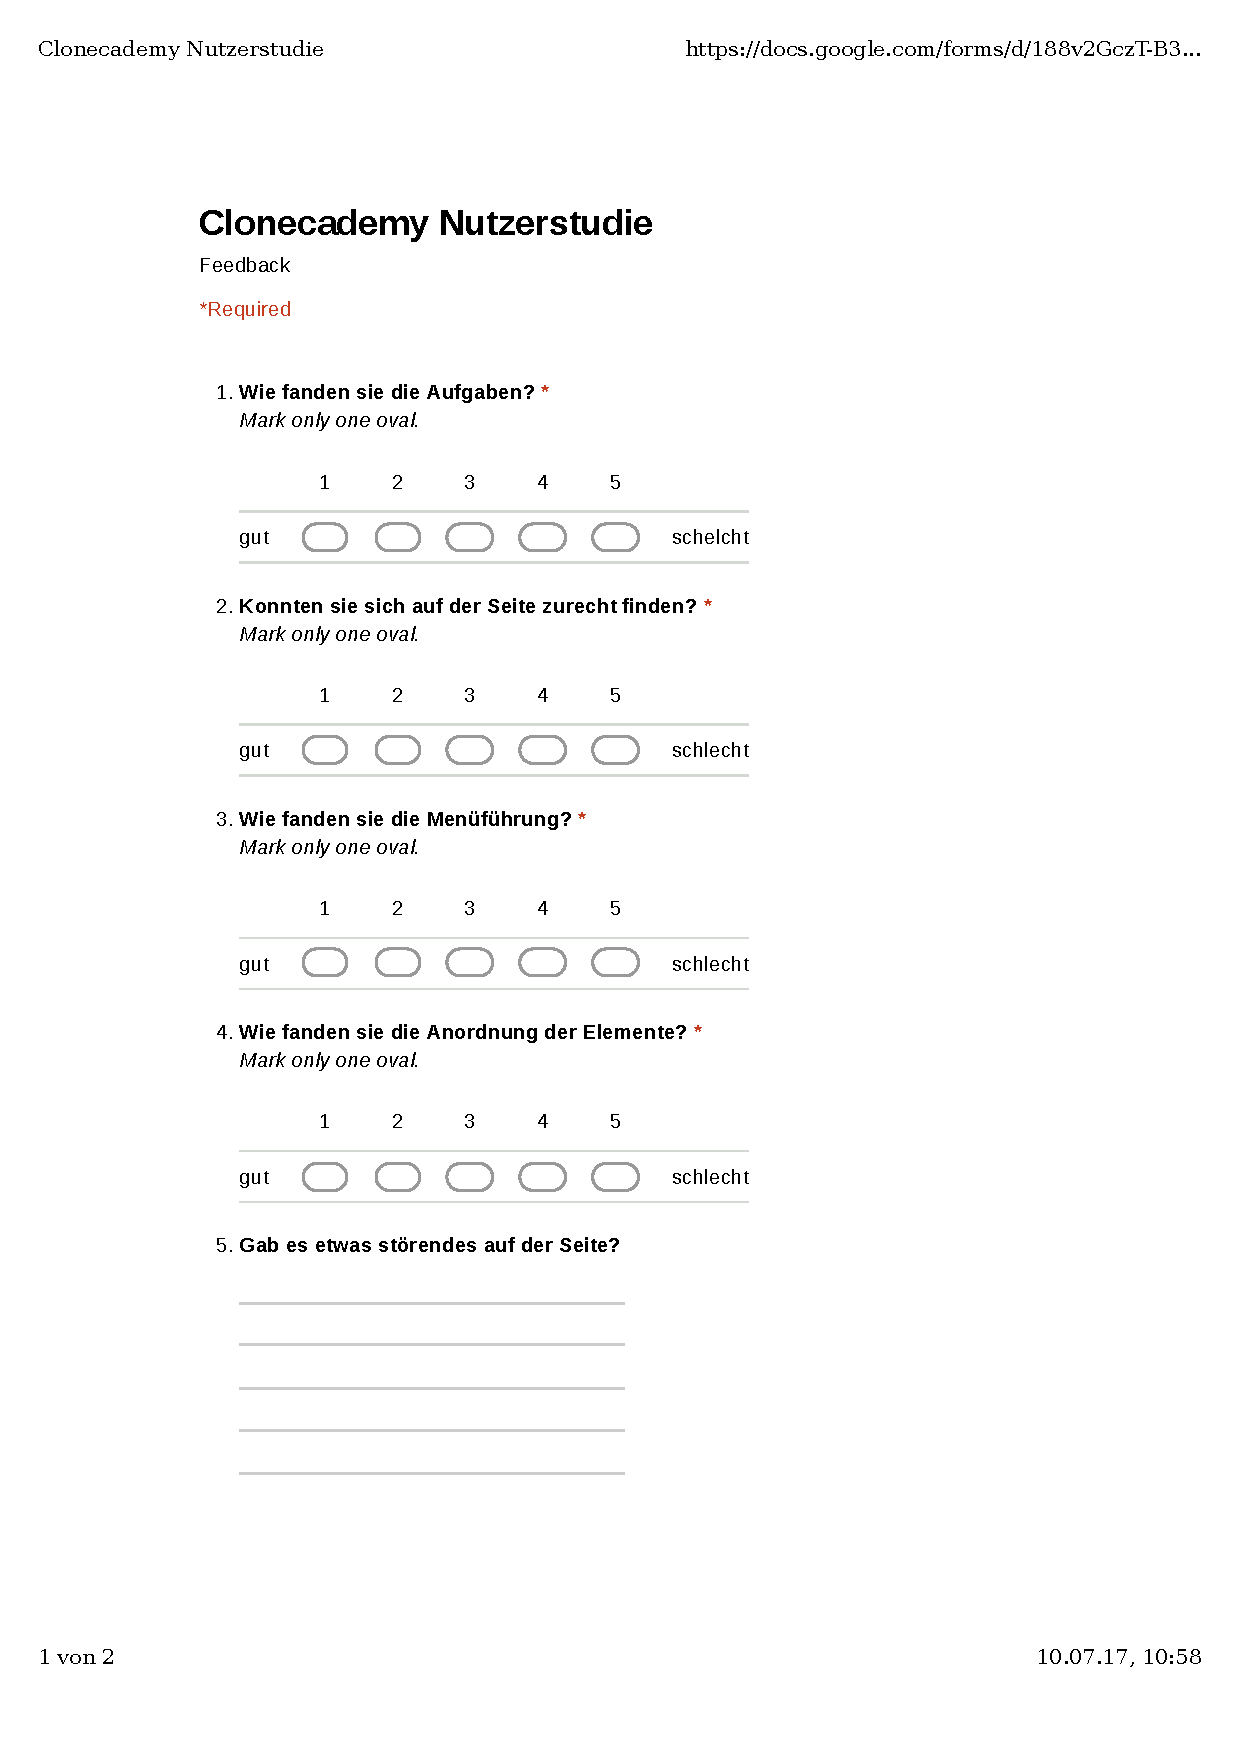
\includepdf[pages=-,pagecommand={},width=\textwidth]{nutzerstudie.pdf}
\end{document}
